\documentclass[11pt,a4paper]{article}

% --- Preamble ---
\usepackage[utf8]{inputenc}
\usepackage[spanish]{babel}
\usepackage[margin=2.5cm]{geometry}
\usepackage{amsmath, amssymb, amsfonts}
\usepackage{graphicx}
\usepackage{booktabs}
\usepackage{hyperref}
\usepackage{caption}
\usepackage{float}

\hypersetup{
    colorlinks=true,
    linkcolor=black,
    pdftitle={Informe Tecnico ENA 2014-2024},
}

\begin{document}

\begin{titlepage}
    \centering
    \vspace*{1cm}
    {\large \textbf{UNIVERSIDAD NACIONAL DEL ALTIPLANO} \par}
    \vspace{0.5cm}
    {\large \textbf{FACULTAD DE INGENIERIA ESTADISTICA E INFORMATICA} \par}
    \vspace{0.4cm}
    {\large \textbf{Escuela Profesional de Ingenieria Estadistica e Informatica} \par}

    \vspace{1.5cm}
    \IfFileExists{logo_unap.png}{
\includegraphics[width=0.35\textwidth]{logo_unap.png}\par}{\vspace{2.6cm}}
    \vspace{1.0cm}

    {\Large \textbf{INFORME TECNICO} \par}
    \vspace{0.5cm}
    {\large \textbf{Analisis Espacial Departamental de la ENA 2014-2024} \par}

    \vfill
    {\large \textbf{Curso:} Estadistica Espacial \par}
    {\large \textbf{Unidad 01 - Tarea 02} \par}
    \vspace{0.6cm}
    {\large \textbf{Presentado por:} Victor Raul Maye Mamani \par}
    {\large \textbf{Codigo:} 217397 \par}
    \vspace{0.6cm}
    {\large \textbf{Docente:} TORRES CRUZ FRED \par}
    \vfill
    {\large Puno, Peru \par}
    {\large \today \par}
\end{titlepage}

\newpage

\begin{abstract}
Este informe presenta un analisis espacial comparativo por departamento usando la Encuesta Nacional Agropecuaria (ENA) para el periodo 2014-2024. El flujo de trabajo integra ingestion y estandarizacion de datos, agregacion estadistica por unidad territorial y union espacial con cartografia departamental. Se reportan cuatro ejes de lectura: fragmentacion de parcelas, dinamica de arrendamiento, uso de abono y gasto en semillas. Los resultados evidencian una heterogeneidad territorial marcada entre costa, sierra y selva, con implicancias directas para la priorizacion de politicas e intervenciones tecnico-productivas.
\end{abstract}

\newpage
\tableofcontents
\newpage

\section{Introduccion}
El analisis espacial aplicado a datos agropecuarios permite pasar de promedios nacionales a diagnosticos territoriales con mayor utilidad para la toma de decisiones. En esta tarea se construye un reporte departamental usando ENA 2014-2024, con variables de estructura productiva y uso de insumos. El objetivo es identificar brechas regionales y traducirlas en decisiones tecnicas concretas, evitando interpretaciones generales que no distingan la diversidad territorial del pais.

\section{Objetivos}
\subsection{Objetivo general}
Caracterizar diferencias agropecuarias entre departamentos del Peru mediante indicadores derivados de la ENA y mapas tematicos comparables.

\subsection{Objetivos especificos}
\begin{itemize}
    \item Estandarizar y consolidar variables seleccionadas de ENA en un formato eficiente para analisis.
    \item Agregar indicadores por departamento para resumir estructura de parcelas, tenencia e intensidad de uso de insumos.
    \item Integrar los resultados con un shapefile departamental y construir mapas interpretables.
    \item Elaborar una lectura tecnica de brechas territoriales con enfoque aplicado.
\end{itemize}

\section{Cumplimiento de la consigna}
Este informe se presenta como entrega unica en PDF y cumple los tres requerimientos solicitados:
\begin{enumerate}
    \item \textbf{Ubicacion espacial de variables ENA (minimo 3):} se presentan cuatro variables con evidencia cartografica.
    \item \textbf{Repositorio GitHub (codigo):} se adjunta enlace oficial del proyecto.
    \item \textbf{URL del portafolio del curso:} se adjunta enlace de despliegue publico.
\end{enumerate}

\subsection{Variables espaciales reportadas}
\begin{table}[H]
\centering
\caption{Variables ENA con representacion espacial en este informe}
\begin{tabular}{@{}lll@{}}
\toprule
\textbf{Variable} & \textbf{Descripcion} & \textbf{Evidencia} \\ \midrule
\texttt{P14\_TOTPARCELAS} & Promedio de parcelas por productor & Figura 1 \\
\texttt{P110\_3} & Prevalencia de arrendamiento agricola & Figura 2 \\
\texttt{P236} & Uso de abono o fertilizante & Figura 3 \\
\texttt{P235} & Gasto en semillas & Figura 4 \\ \bottomrule
\end{tabular}
\end{table}

\section{Datos y metodologia}
\subsection{Fuentes}
\begin{itemize}
    \item Base ENA 2014-2024 (archivo \texttt{.sav}) procesada localmente.
    \item Cartografia departamental del Peru (shapefile).
\end{itemize}

\subsection{Variables principales}
\begin{itemize}
    \item \texttt{P14\_TOTPARCELAS}: promedio de parcelas por productor.
    \item \texttt{P110\_3}: condicion de arrendatario.
    \item \texttt{P236}: uso de abono o fertilizante.
    \item \texttt{P235}: gasto en semilla.
\end{itemize}

\subsection{Flujo de procesamiento}
El procedimiento se ejecuto con scripts en R: (i) ingestion y conversion a Parquet, (ii) limpieza y agregacion con \texttt{data.table}, (iii) union espacial con \texttt{sf} y (iv) construccion de mapas en \texttt{ggplot2}. La cartografia y la tabla de indicadores se homogeneizaron por nombre de departamento para asegurar un emparejamiento correcto en el \textit{join} espacial.

\section{Resultados}
\subsection{Fragmentacion de parcelas}
La fragmentacion es mayor en la sierra sur. Huancavelica (4.94) y Puno (4.58) muestran los promedios mas altos de parcelas por productor, mientras que Lima (1.44) y Lambayeque (1.64) presentan unidades mas consolidadas. Esta diferencia sugiere que, en la sierra sur, la gestion operativa se dificulta por dispersion predial; por tanto, resultan pertinentes estrategias de mecanizacion para pequena escala y esquemas de coordinacion entre productores.

\begin{figure}[H]
    \centering
    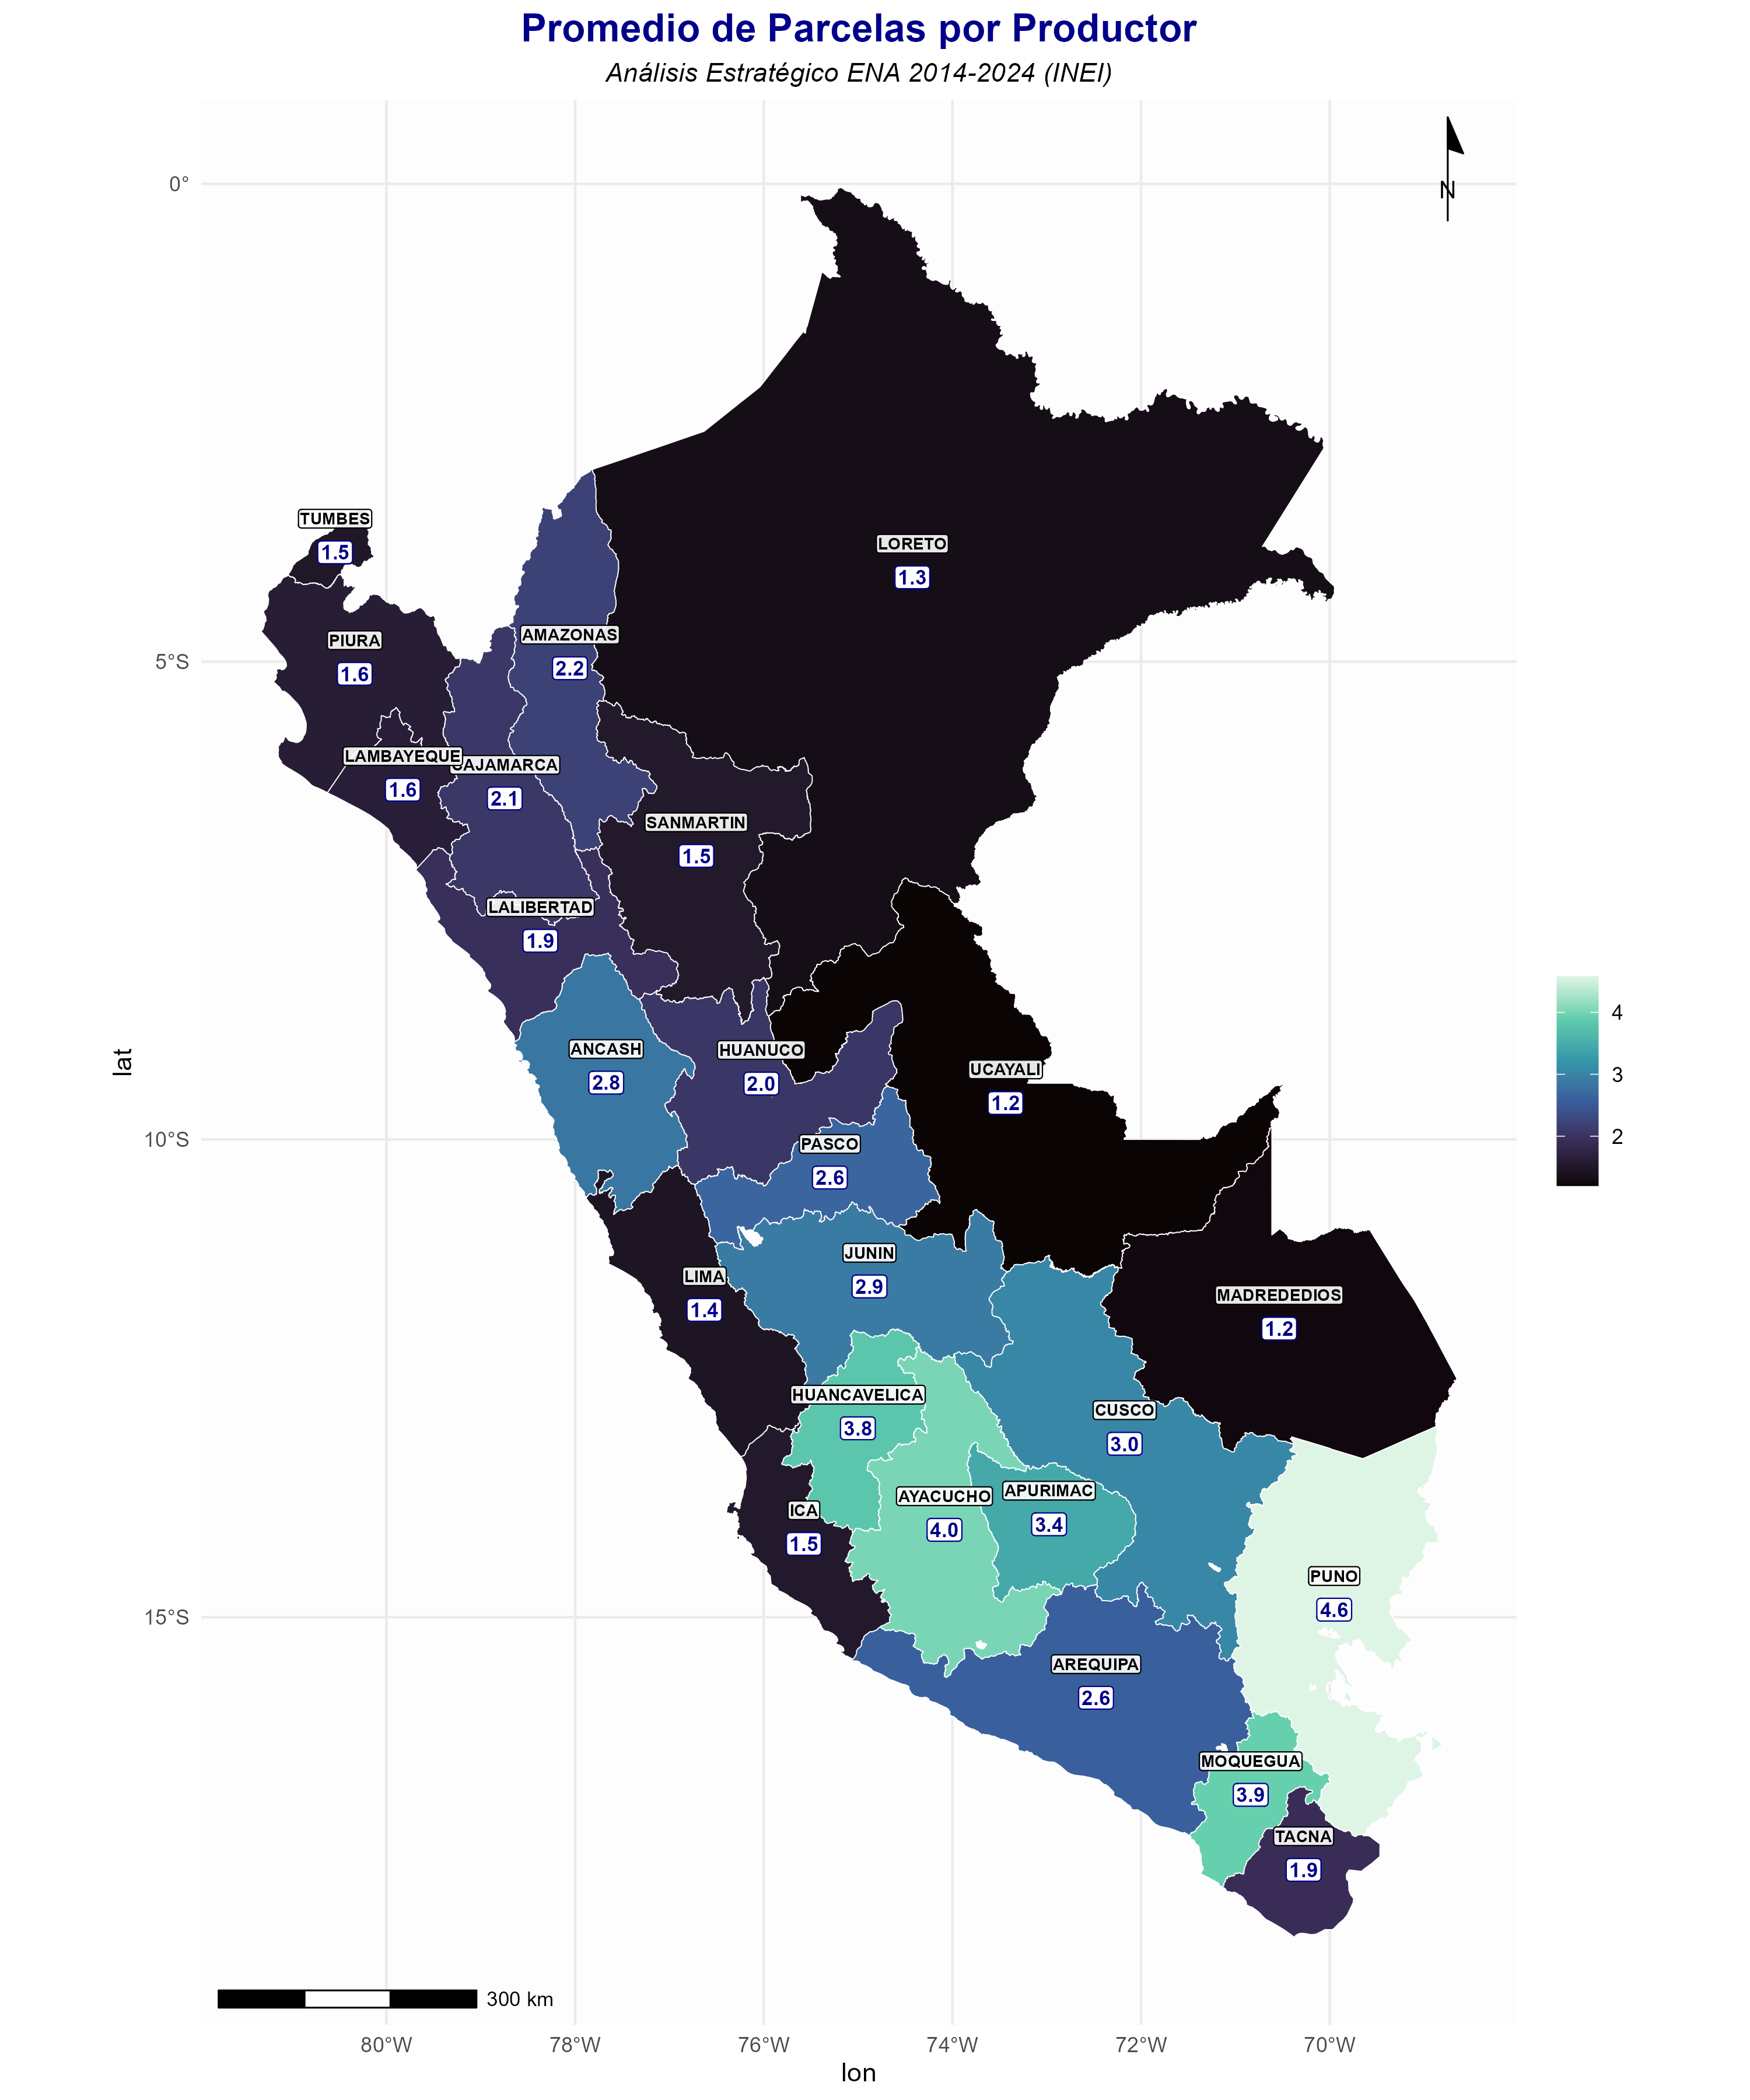
\includegraphics[width=0.82\textwidth]{../results/mapa_01_parcelas.png}
    \caption{Promedio de parcelas por productor (ENA 2014-2024).}
\end{figure}

\subsection{Arrendamiento agricola}
El arrendamiento es mas dinamico en Lima (18.3), Junin (17.3) y Arequipa (15.1). En contraste, Loreto (0.5) y Ucayali (2.7) muestran mercados de tierras poco activos. La lectura operativa es clara: donde el arrendamiento es alto, la produccion presenta mayor rotacion y menor horizonte de inversion de largo plazo; en consecuencia, los instrumentos de financiamiento de campana y los seguros de corto plazo son mas pertinentes.

\begin{figure}[H]
    \centering
    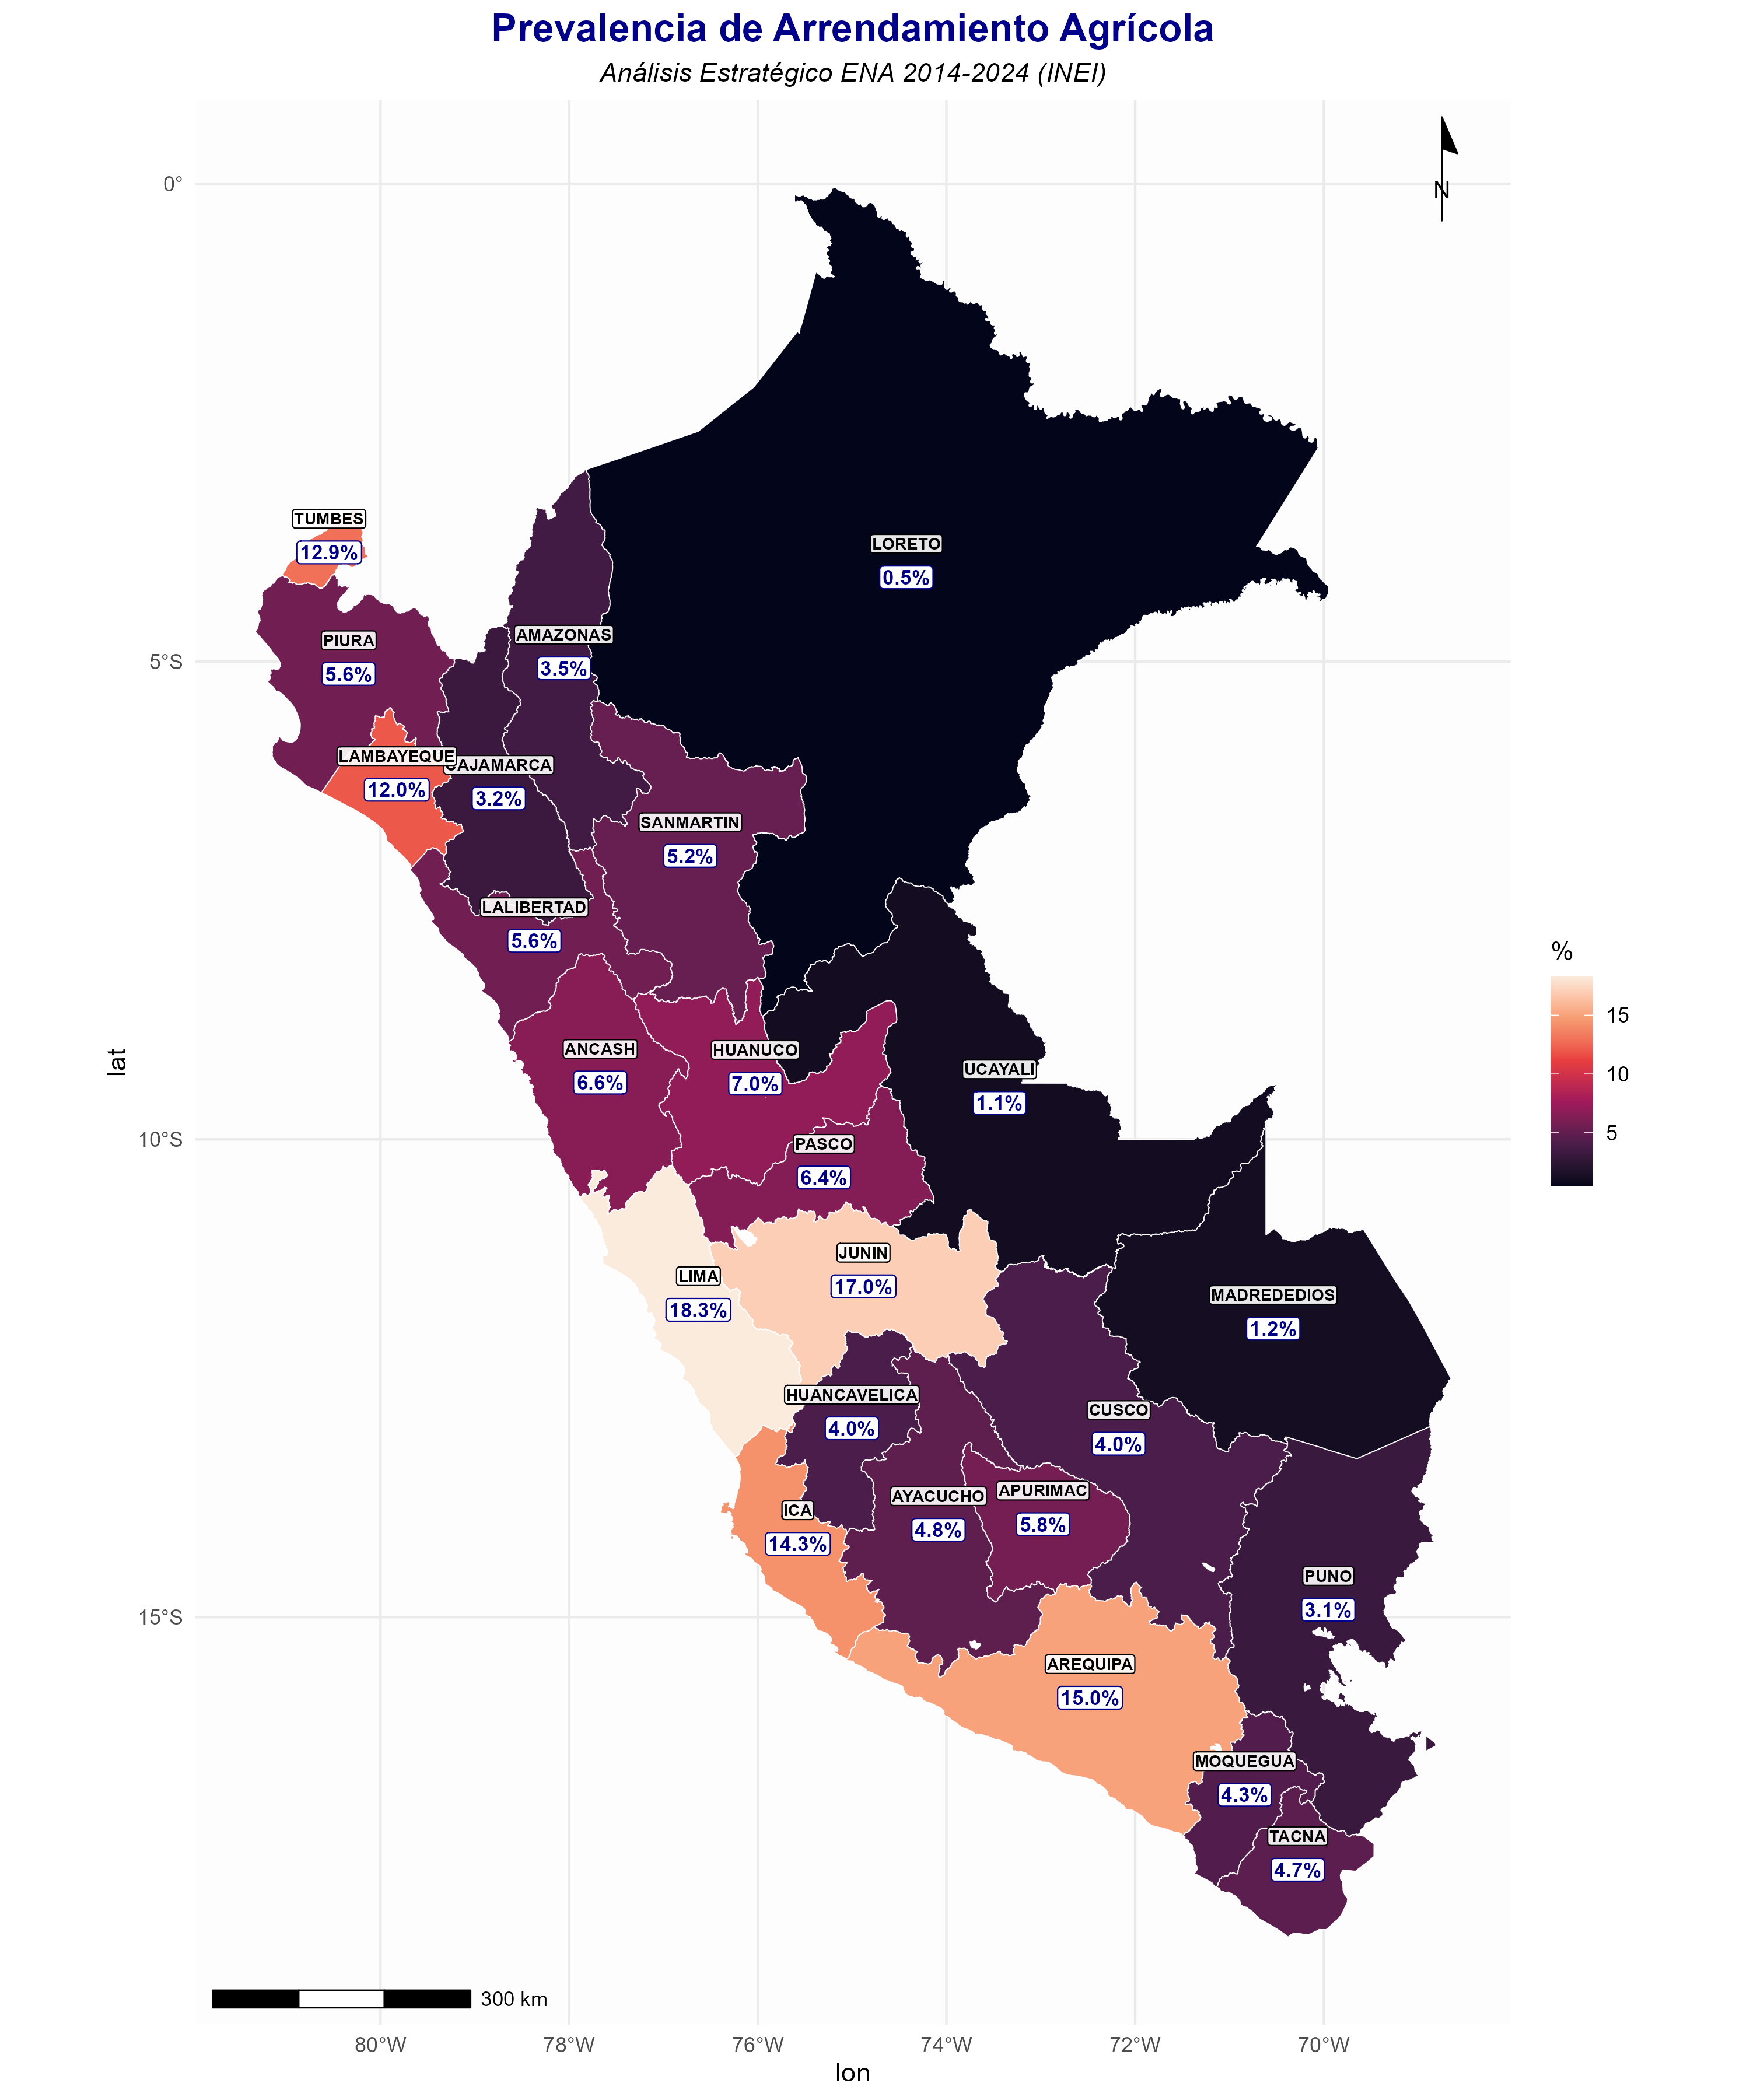
\includegraphics[width=0.82\textwidth]{../results/mapa_02_arrendamiento.png}
    \caption{Prevalencia de arrendamiento agricola por departamento.}
\end{figure}

\subsection{Uso de abono}
Existe una brecha marcada entre selva baja y sierra central/sur. Loreto (2.2\%) y Ucayali (4\%) tienen uso bajo de abono, mientras Huancavelica (72.4\%) y Junin (62.5\%) muestran uso alto. La interpretacion tecnica indica que no se trata solo de acceso al insumo, sino tambien de distinta intensidad tecnologica y de practicas agronomicas. En selva, la prioridad es la adopcion basica; en sierra, la prioridad es la eficiencia de dosis y la calidad del manejo.

\begin{figure}[H]
    \centering
    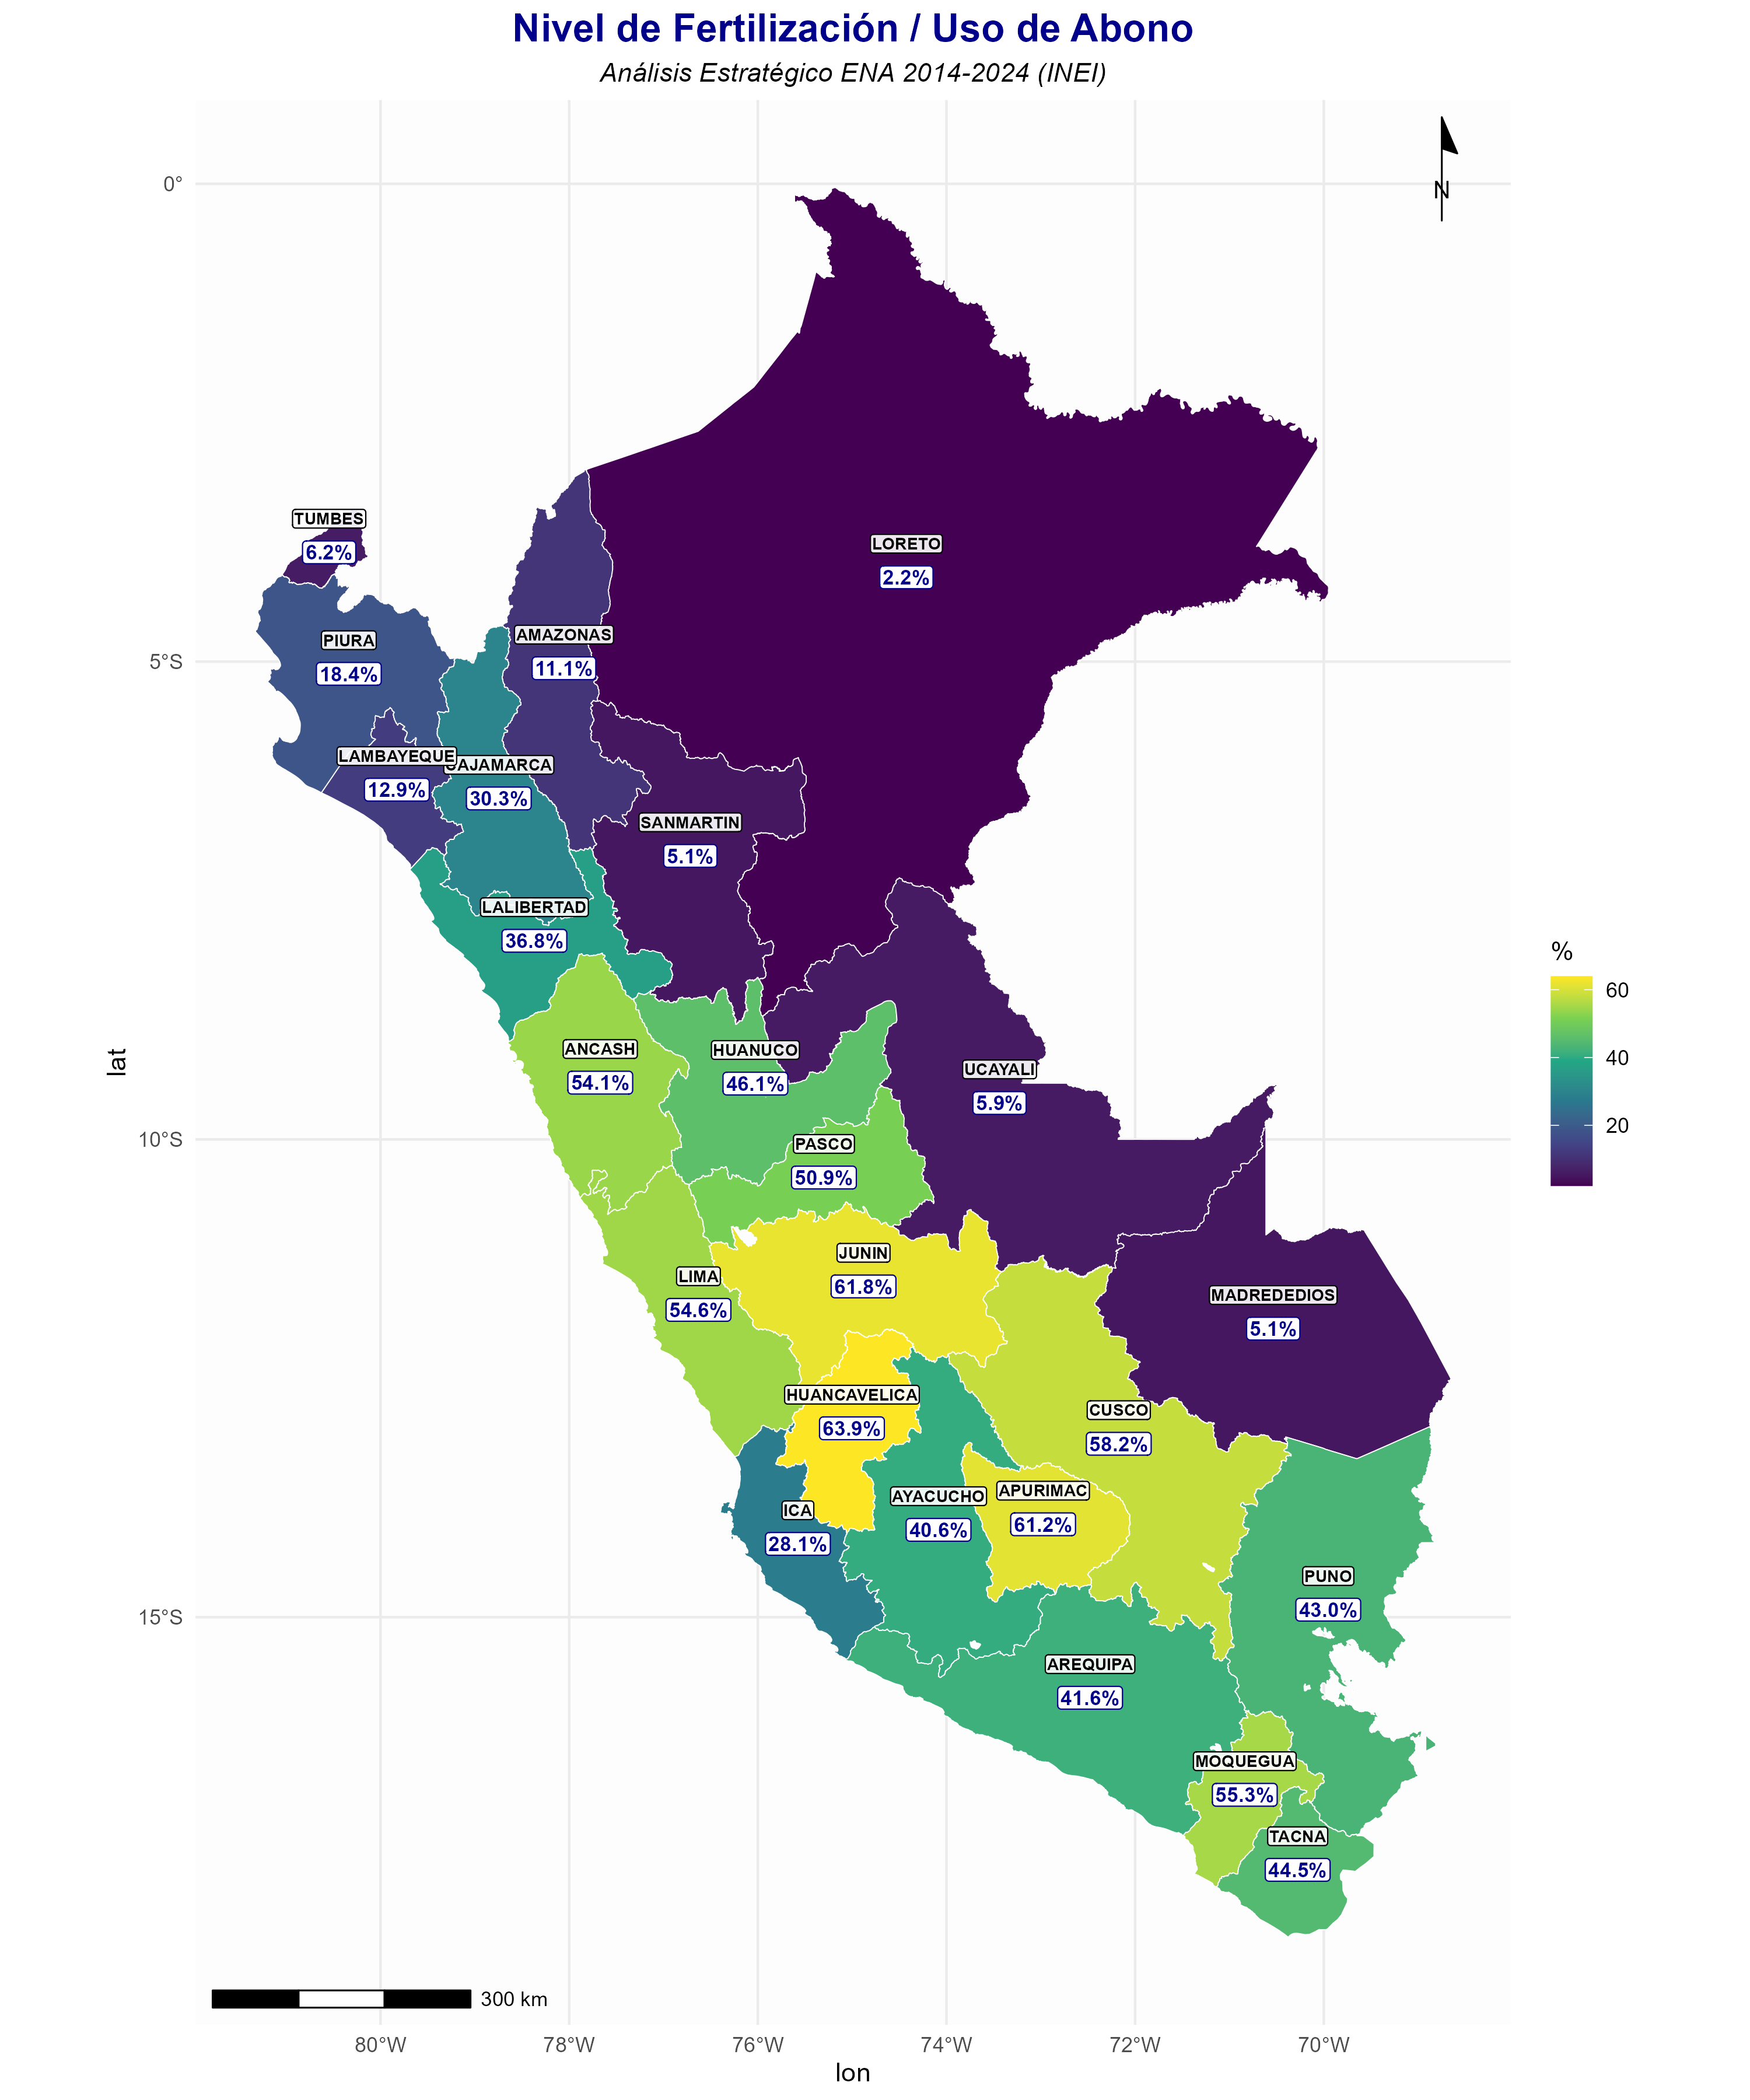
\includegraphics[width=0.82\textwidth]{../results/mapa_03_abono.png}
    \caption{Uso de abono o fertilizante por departamento.}
\end{figure}

\subsection{Gasto en semillas}
La compra de semillas es casi total en Junin (99.8\%) y Apurimac (99.2\%), mientras Ucayali (61.8\%) conserva una proporcion mas alta de productores que no compran semilla certificada. Esto sugiere dos escenarios: en departamentos con gasto alto, el foco no es introducir la compra, sino mejorar la calidad de semilla; en departamentos con gasto medio, el cuello de botella principal sigue siendo el acceso comercial y la logistica de distribucion.

\begin{figure}[H]
    \centering
    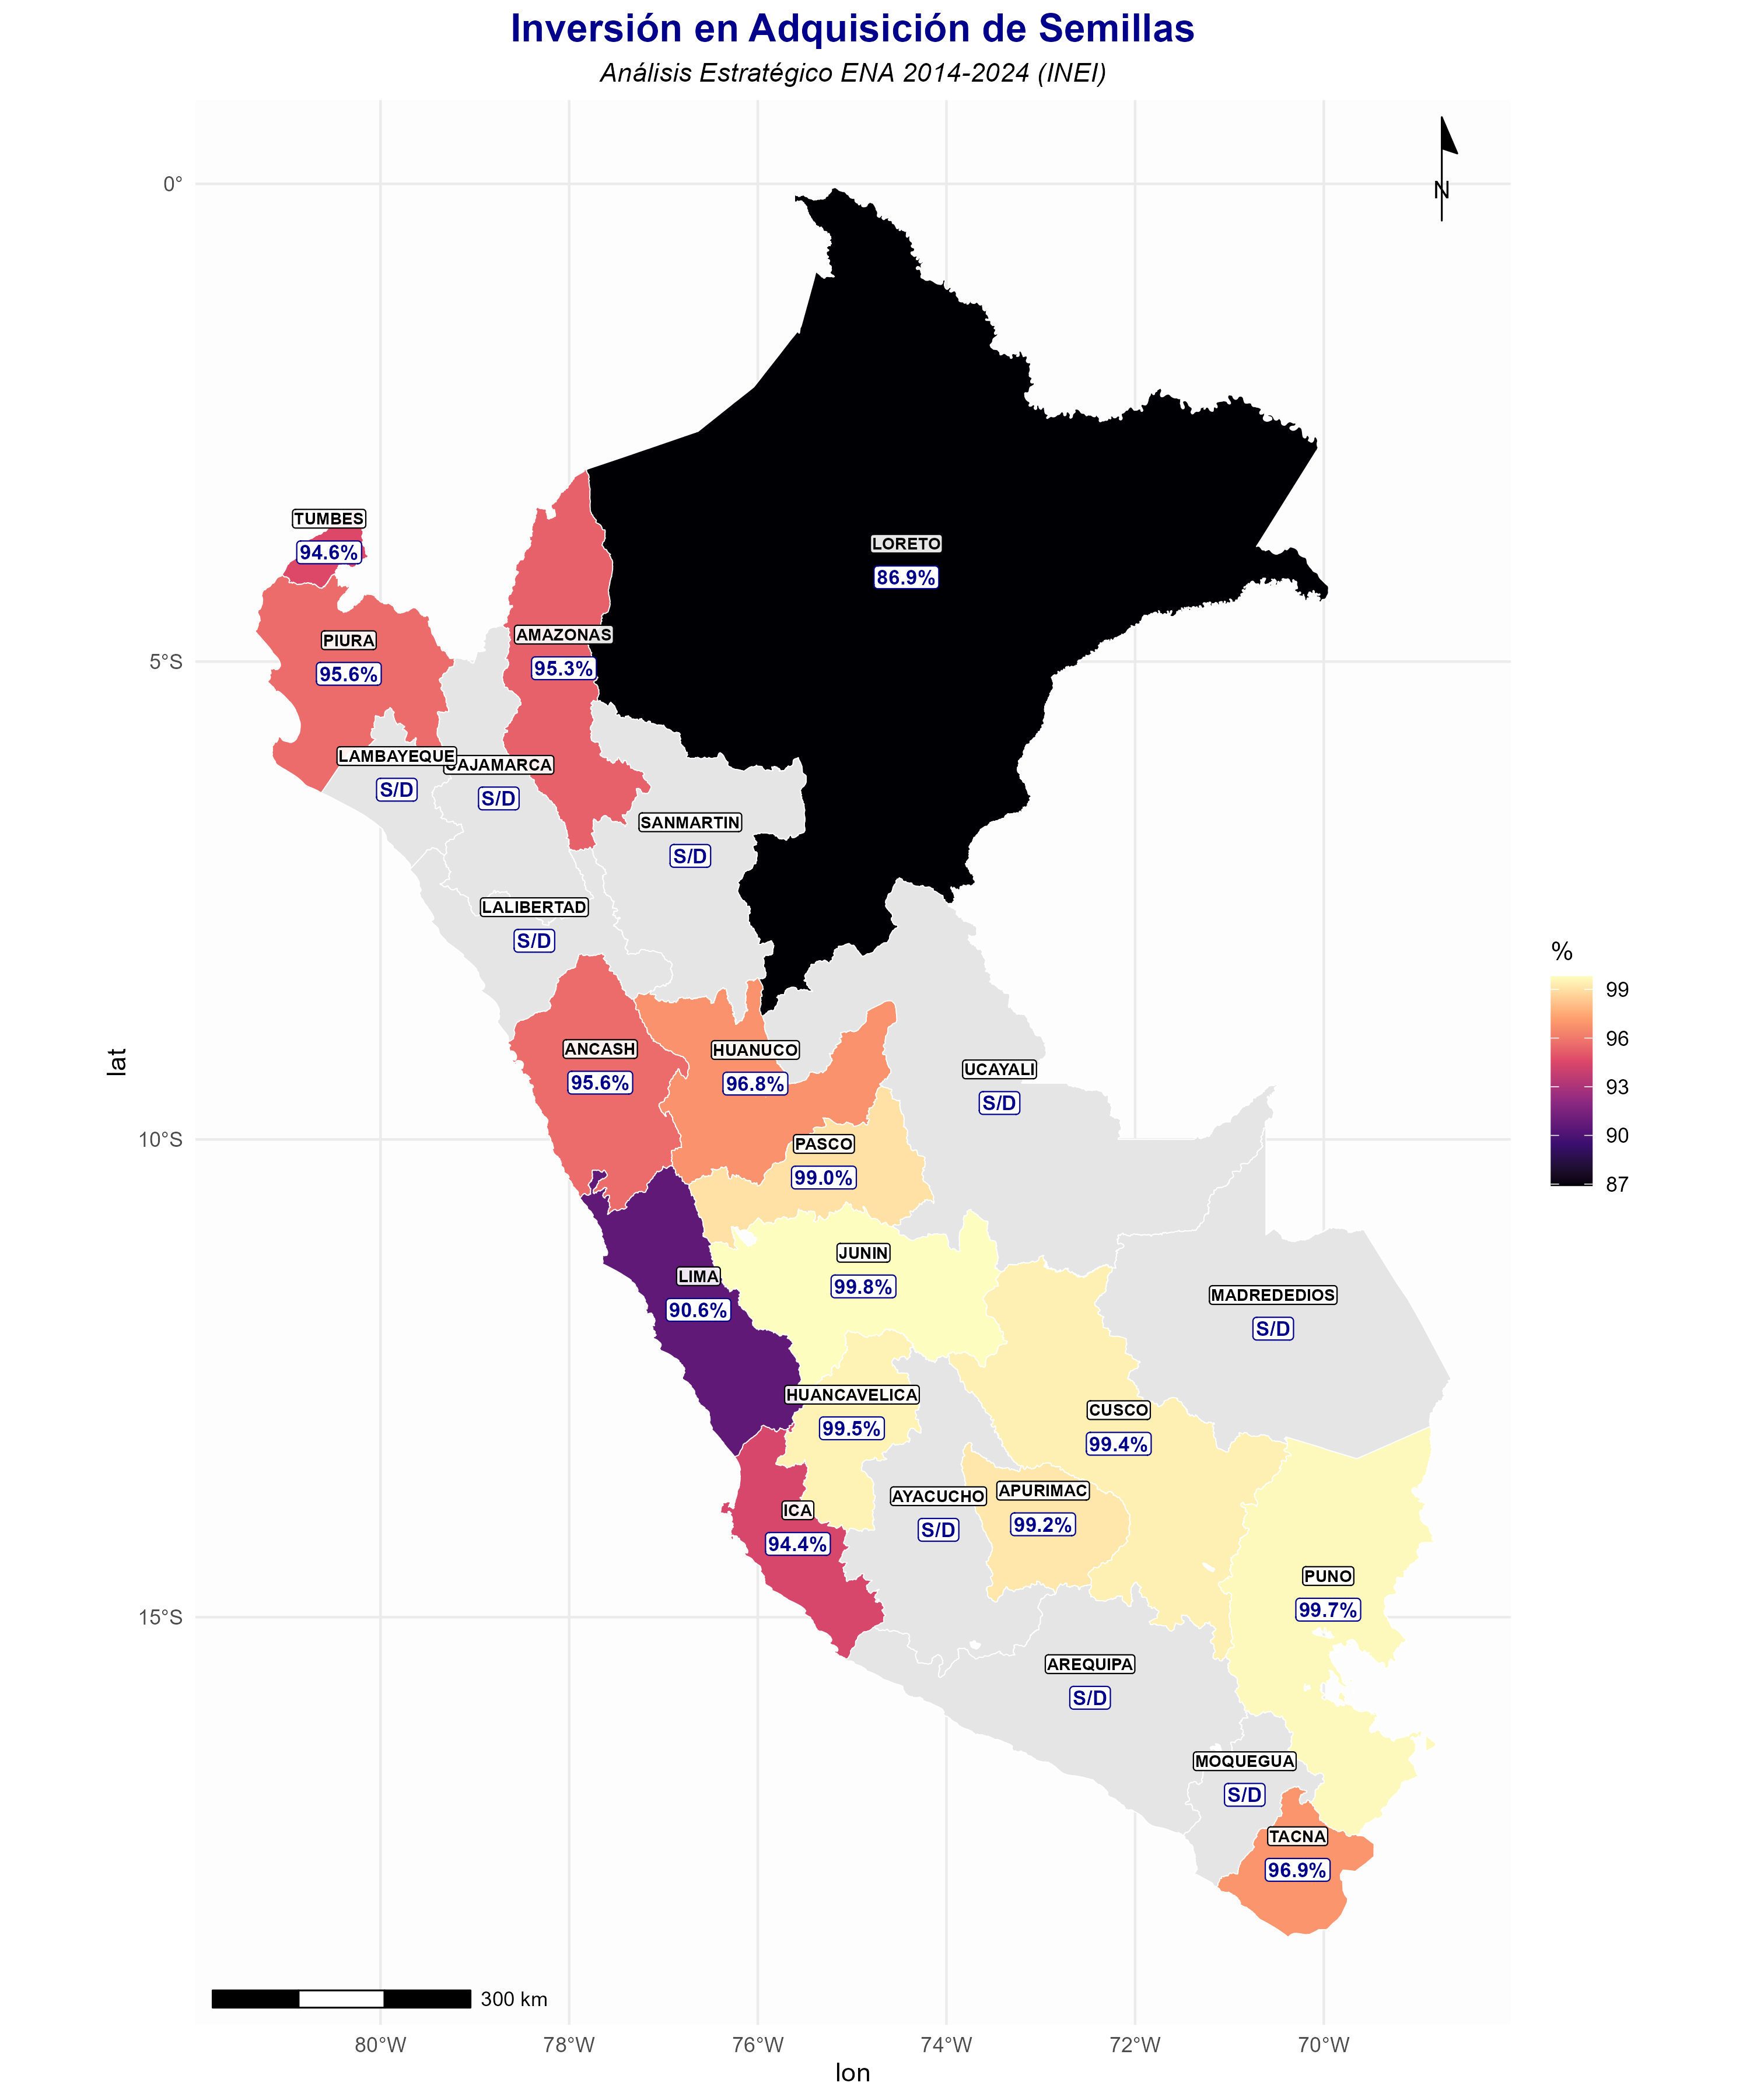
\includegraphics[width=0.82\textwidth]{../results/mapa_04_semillas.png}
    \caption{Gasto en semillas por departamento.}
\end{figure}

\section{Discusion tecnica}
Los resultados confirman que la variabilidad espacial no es ruido, sino estructura informativa del fenomeno agropecuario. Una estrategia unica nacional pierde precision al no distinguir perfiles regionales. En este caso, los patrones observados permiten segmentar decisiones: (i) departamentos con alta fragmentacion requieren soluciones de pequena escala; (ii) departamentos con alto arrendamiento requieren instrumentos financieros de ciclo corto; (iii) departamentos con baja adopcion de abono necesitan programas de entrada tecnologica; y (iv) departamentos con alta compra de semilla requieren enfasis en calidad y rendimiento.

\section{Conclusiones}
\begin{itemize}
    \item El analisis departamental ENA 2014-2024 identifica brechas espaciales consistentes en estructura productiva y uso de insumos.
    \item La combinacion de procesamiento tabular y cartografia tematica permite pasar de datos a decisiones concretas por territorio.
    \item Priorizacion sugerida: Junin y Lima para servicios financieros y tecnologia; Sierra Sur (Puno y Huancavelica) para logistica y pequena mecanizacion; y Selva como frente de expansion con enfoque en adopcion basica de insumos.
\end{itemize}

\section{Enlaces de verificacion}
\begin{itemize}
    \item Repositorio GitHub (codigo): \href{https://github.com/valec3/unap-spatial-statistics}{https://github.com/valec3/unap-spatial-statistics}
    \item Portafolio del curso: \href{https://victor-maye-est334.vercel.app/}{https://victor-maye-est334.vercel.app/}
\end{itemize}

\section{Anexo de reproducibilidad}
Scripts principales utilizados:
\begin{itemize}
    \item \texttt{../00\_setup.R}
    \item \texttt{../01\_ingestion.R}
    \item \texttt{../02\_processing.R}
    \item \texttt{../03\_reporting.R}
    \item \texttt{../master.R}
\end{itemize}

\end{document}
